\documentclass{article}
\usepackage{geometry}
\usepackage{amsmath}
\usepackage{amssymb}
%\usepackage{multirow}
\usepackage{fancyhdr}
%\usepackage{colortbl}
%\usepackage{enumitem}
\usepackage{tikz}
\usetikzlibrary{calc,trees,positioning,arrows,fit,shapes,calc}
\tikzset{>=latex}
%\usepackage{textcomp}
\pagestyle{fancy}

\lhead{MATH381.004 --- Homework 8}
\rhead{\textbf{Jason He}}

% 9.1:  1e), 2, 3a)c)e),  4, 6d)e)f), 7, 10, 34, , 40

% 9.5:   1 a)b)c), 3

\begin{document}
\begin{enumerate}
    \item[{[\S 9.1]} 1e.] $\{ (0,1), (1,0), (1,1), (1,2), (1,3), (2,1), (2,3), (3,1), (3,2), (4,1), (4,3) \}$
    \item[2.]
        \begin{itemize}
            \item[(a)] $(1,1), (1,2), (1,3), (1,4), (1,5), (1,6), (2,2), (2,4), (2,6), (3,3), (3,6), (4,4), (5,5), (6,6)$
            \item[(b)] \hfill

            %\begin{figure}[h]
             %\centering
             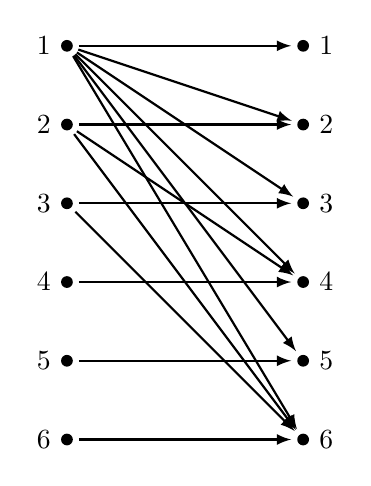
\begin{tikzpicture}[ele/.style={fill=black,circle,minimum width=1pt,inner sep=1.5pt}]
              \node[ele,label=left:$1$] (a1) at (0,6) {};    
              \node[ele,label=left:$2$] (a2) at (0,5) {};    
              \node[ele,label=left:$3$] (a3) at (0,4) {};
              \node[ele,label=left:$4$] (a4) at (0,3) {};
              \node[ele,label=left:$5$] (a5) at (0,2) {};
              \node[ele,label=left:$6$] (a6) at (0,1) {};              

              \node[ele,label=right:$1$] (b1) at (3,6) {};    
              \node[ele,label=right:$2$] (b2) at (3,5) {};    
              \node[ele,label=right:$3$] (b3) at (3,4) {};
              \node[ele,label=right:$4$] (b4) at (3,3) {};
              \node[ele,label=right:$5$] (b5) at (3,2) {};
              \node[ele,label=right:$6$] (b6) at (3,1) {}; 
 
              \draw[->,thick,shorten <=2pt,shorten >=2pt] (a1) -- (b1);
              \draw[->,thick,shorten <=2pt,shorten >=2pt] (a1) -- (b2);
              \draw[->,thick,shorten <=2pt,shorten >=2pt] (a1) -- (b3);
              \draw[->,thick,shorten <=2pt,shorten >=2pt] (a1) -- (b4);
              \draw[->,thick,shorten <=2pt,shorten >=2pt] (a1) -- (b5);
              \draw[->,thick,shorten <=2pt,shorten >=2pt] (a1) -- (b6);
              \draw[->,thick,shorten <=2pt,shorten >=2pt] (a2) -- (b2);
              \draw[->,thick,shorten <=2pt,shorten >=2pt] (a2) -- (b4);
              \draw[->,thick,shorten <=2pt,shorten >=2pt] (a2) -- (b6);
              \draw[->,thick,shorten <=2pt,shorten >=2pt] (a3) -- (b3);
              \draw[->,thick,shorten <=2pt,shorten >=2pt] (a3) -- (b6);
              \draw[->,thick,shorten <=2pt,shorten >=2pt] (a4) -- (b4);
              \draw[->,thick,shorten <=2pt,shorten >=2pt] (a5) -- (b5);
              \draw[->,thick,shorten <=2pt,shorten >=2pt] (a6) -- (b6);
             \end{tikzpicture}
            %\end{figure}

            \item[(c)] \hfill

                \begin{tabular}{c|cccccc}
                $R$ & 1 & 2 & 3 & 4 & 5 & 6 \\\hline
                1 & $\times$ & $\times$ & $\times$ & $\times$ & $\times$ & $\times$ \\
                2 & & $\times$ & & $\times$ & & $\times$ \\
                3 & & & $\times$ & & & $\times$ \\
                4 & & & & $\times$ & & \\
                5 & & & & & $\times$ & \\
                6 & & & & & & $\times$
                \end{tabular}
        \end{itemize}
    \item[3.]
        \begin{itemize}
            \item[(a)] Transitive
            \item[(c)] Symmetric
            \item[(e)] Reflexive, symmetric, antisymmetric, and transitive
        \end{itemize}
    \item[4.]
        \begin{itemize}
            \item[(a)] Antisymmetric and transitive
            \item[(b)] Reflexive, symmetric, and transitive
            \item[(c)] Reflexive, symmetric, and transitive
            \item[(d)] Reflexive and symmetric
        \end{itemize}
    \item[6.]
        \begin{itemize}
            \item[(d)] Antisymmetric
            \item[(e)] Reflexive and symmetric
            \item[(f)] Symmetric
        \end{itemize}
    \item[7.]
        \begin{itemize}
            \item[(a)] Symmetric
            \item[(b)] Symmetric and transitive
            \item[(c)] Symmetric
            \item[(d)] Reflexive, symmetric, and transitive
            \item[(e)] Reflexive and transitive
            \item[(f)] Reflexive, symmetric, and transitive
            \item[(g)] Antisymmetric
            \item[(h)] Antisymmetric and transitive
        \end{itemize}
    \item[10.]
        \begin{itemize}
            \item[(a)] $\{ (0,0), (1,1), (2,2) \}$ on $\{ 0,1,2 \}$
            \item[(b)] $\{ (0,1), (1,0), (0,2) \}$ on $\{ 0,1,2 \}$
        \end{itemize}
    \item[34.]
        \begin{itemize}
            \item[(a)] $R_6$
            \item[(b)] $R_2$
            \item[(c)] $R_5$
            \item[(d)] $\emptyset$
            \item[(e)] $\emptyset$
            \item[(f)] $R_5$
            \item[(g)] $R_6$
            \item[(h)] $R_6$
        \end{itemize}
    \item[40.]
        \begin{itemize}
            \item[(a)] $\{ (a,b) \mid a \text{ divides or is a multiple of } b \}$
            \item[(b)] $\{ (a,b) \mid a \text{ divides and is a multiple of } b \}$
            \item[(c)] $\{ (a,b) \mid a \text{ divides but is not a multiple of } b \}$
            \item[(d)] $\{ (a,b) \mid a \text{ does not divide but is a multiple of } b \}$
            \item[(e)] $\{ (a,b) \mid a \text{ divides or is a multiple of } b \text{, but not both} \}$
        \end{itemize}
    \item[{[\S 9.5]} 1.]
        \begin{itemize}
            \item[(a)] Yes
            \item[(b)] No --- lacking reflexivity and transitivity
            \item[(c)] Yes
        \end{itemize}
    \item[3.]
        \begin{itemize}
            \item[(a)] Yes
            \item[(b)] No --- lacking transitivity
            \item[(c)] No --- lacking reflexivity, symmetry, and transitivity
            \item[(d)] Yes
            \item[(e)] No --- lacking reflexivity and transitivity
        \end{itemize}
\end{enumerate}
\end{document}